\section{Архитектура и модули системы} % (fold)
\label{sec:arch_and_mod}

Разработанное программное обеспечение представляет из себя библиотеку кода написанную на языках \fsharp{} и \csharp{}.
Библиотека предназначена для представления модификации классических байесовых сетей, упомянутой на странице~\pageref{page:domain:bayes_mod} в подразделе~\ref{sub:domain:bayes_net}.

\subsection{Типы для работы с графами}
\label{sub:arch_and_mod:graphlib}

Так как в дипломном проекте рассматривается одна из разновидностей графовых моделей, то, очевидно, для представления таких моделей в разрабатываемой библиотеке должна быть часть, отвечающая за представление и работу с графами.
При реализации здесь было несколько альтернативных путей: использовать одну из доступных библиотек для платформы \dotnet{} для работы с графами или реализовать собственную.
Среди готовых библиотек можно было бы использовать QuickGraph\footnote{\url{http://quickgraph.codeplex.com/}}, Directed Graph for .NET\footnote{\url{http://directedgraph4net.codeplex.com/}} или GrapheNET\footnote{\url{http://graphenet.codeplex.com/}}.
Но было принято решение остановиться на варианте, подразумевающем разработку собственных типов для работы с графами.
Это решение было обосновано тем, что вышеуказанные библиотеки являются сложными и содержат в себе очень много функциональности не нужной для решения поставленных задач, в дополнение не было приобретено лишних мегабайтовых внешних зависимостей для библиотеки.

Одним из важных решений, которое было принято в начале проектирования модуля работы с графами, было использование по возможности неизменяемых структур данных.
Это решение выгодно отличает разработанную реализацию от существующих библиотек, от использования которых было принято решение отказаться. 
Существующие библиотеки ориентированы на работу в императивном стиле и с изменяемым состоянием.
Также использование неизменяемых структур данных для реализации типов для представления графов в дальнейшем положительно сказалось на простоте реализации поиска структуры вероятностной сети в алгоритмах вывода структуры по данным.
Часть разрабатываемой библиотеки, содержащая типы для работы с графами, реализована на языке программирования \fsharp{}.
Краткое описание основных особенностей данного языка приведено в подразделе~\ref{sub:practice:fsharp_overview}.
Решение использовать данный язык было продиктовано желанием сократить количество возможных ошибок и размер кодовой базы, необходимой для реализации поставленной задачи, а так же желанием применить в <<боевых>> условиях язык программирования с хорошей поддержкой функционального программирования.

Внутренним представлением графа является неизменяемый словарь, содержащий вложенный неизменяемый мульти"=словарь\footnote{Словарь позволяющий хранить множество значений с одинаковым ключом.}.
Основные определения структуры данных графа приведены в листинге~\ref{lst:arch_and_mod:graph_definition}:
\begin{lstlisting}[style=fsharpstyle,caption={Определение структуры данных для представления графа}, label=lst:arch_and_mod:graph_definition]
/// Graph arc 
type Arc<'T> =
    | Outgoing of 'T
    | Incoming of 'T

/// Immutable Graph class
[<ReferenceEquality; NoComparison>]
type Graph<'Vertex, 'Arc when 'Vertex : comparison and 'Vertex : equality and 'Vertex :> IComparable> = 
    private Graph of Map<'Vertex, MultiMap<'Vertex, Arc<'Arc>>>
\end{lstlisting}

Данная структура данных для представления графа подходит для работы как с неориентированными так и с ориентированными мультиграфами.
Воспринимать граф как ориентированный или нет задача конкретного алгоритма, работающего с графом.
Разработанная библиотека для представления графа предоставляет необходимые операции для манипулирования структурой графа. 
Библиотека также предоставляет небольшое количество алгоритмов для работы с графами, необходимых в рамках решения задач, возникающих при поиске структуры вероятностной сети.
В частности реализованы алгоритмы топологической сортировки, поиска в глубину и ширину, поиска сильно"=связанных компонетов и проверки графа на наличие направленных циклов. 

Одной из особенностей разработанной библиотеки является ориентированность на использование как из языка \fsharp{} в <<функциональном стиле>>, так и из языка \csharp{} "--- в <<императивном>>.
Для реализации данной возможности были учтены рекомендации приведенные в~\cite{fsdg_2010}.
Функциональность разработанной библиотеки покрыта большим набором модульных тестов, написанных с использованием библиотек xUnit\footnote{\url{http://xunit.codeplex.com/}} и Unquote\footnote{\url{http://code.google.com/p/unquote/}}.


\subsection{Представление вероятностной сети}
\label{sub:arch_and_mod:probab_net}

Другой важной частью разработанной библиотеки являются типы для представления и работы с самими вероятностными сетями.
Первостепенными требованиями, поставленными перед началом проектирования типов, были следующие пункты:
\begin{itemize}
  \item Типы предназначены для представления модификации классических байесовых сетей, упомянутой в разделе~\ref{sub:domain:bayes_net} на странице~\pageref{page:domain:bayes_mod}.
  \item Представление сети должно быть <<многослойным>>.
  Под <<многослойностью>> понимается возможность расширения представления сети дополнительными <<слоями>> атрибутов, с целью увеличения количества сценариев, в которых данные типы пригодны к использованию.
  Например, в случае когда нужно знать лишь структуру сети можно использовать лишь информацию о структуре "--- граф.
  Для проведения статистического вывода суждений добавляется дополнительный <<слой>>, содержащий талицы условных и безусловных вероятностей.
  В случаях, когда нужно отображать сеть пользователю, добавляется еще один <<слой>>, содержащий дополнительную информацию о переменных и их состояниях. 
  \item Сеть должна предоставлять возможность отмены вносимых в нее изменений, т.\,е. по сути поддерживать версионность.
  \item Сеть должна предоставлять возможность валидации её структуры. 
\end{itemize}

Приняв во внимание приведенные выше требования были приняты следующие решения:
\begin{itemize}
  \item Необходимо разработать отдельные типы для представления вершин вероятностной модели и связей между переменными в этой модели.
  В разработанной библиотеке за это отвечают типы \lstinline!Node<'T>! и \lstinline!Link<'T>!, содержащие информацию о переменных, таблицы распределения и дополнительные атрибуты.
  Использование параметрического полиморфизма в реализации данных типов играет ключевую роль в обеспечении <<многослойности>> и расширяемости представления вероятностной сети.
  \item Необходимы типы для представления распределения.
  В предложенной реализации был разработан тип для представления безусловного распределения случайной величины, эта таблица хранится в сети как один из аттрибутов типа \lstinline!Node<'T>!, и тип для представления условного распределения пары случайных величин, экземпляр данного типа хранится как аттрибут связи между переменными "--- \lstinline!Link<'T>!.
  Было сочтено целесообразным в качестве внутренней реализации таблиц распределения использовать готовую библиотеку для работы с матрицами и другими математическими объектами и понятиями "--- Math.NET Numerics\footnote{\url{http://numerics.mathdotnet.com/}}.
  Соответственно в предложенной реализации использовались типы \lstinline!Vector<float>! и \lstinline!Matrix<float>! и сопутствующие операции над ними.
  Использование данной библиотеки позволило сократить объём сопутствующего кода, необходимого для реализации библиотеки для работы с вероятностными сетями, также уменьшив множество потенциальных ошибок реализации.
  В данном случае преимущества от использования библиотеки превысили затраты на добавление и поддержку дополнительных зависимостей.

  \item Требование возможности отмены изменений вносимых в вероятностную сеть привело к реализации сети, как и в случае типов для представления графов, к реализации сети как неизменяемой структуры данных.
  Все операции, при условии использования специальных функций, возвращают новый экземпляр сети, оставляя старый не изменённым.
  Подобная реализация типов автоматически дает возможность производить версионирование экземпляров типа, т.\,к. всегда есть доступ к изменённой копии и исходному экземпляру.
  С первого взгляда данный подход кажется очень расточительным по памяти, но на самом деле оказывается, что все с точностью до наоборот, т.\,к. обычно, и в данном конкретном случае, при модификации неизменяемой структуры данных большая часть структуры разделяется между копией и исходной структурой, а физически копирование памяти происходит лишь в тех местах, которые действительно необходимо было поменять.
  Для убедительности, сказанное проиллюстрировано на рисунке~\ref{fig:arch_and_mod:probab_net:immutable_ds_modification}.

  \item Валидация сети происходит на этапе её построения и модификации.
  Дополнительно существуют функции для проверки структуры сети на ацикличность.
  Ацикличность ориентированного графа проверяется с помощью алгоритма нахождения компонент сильной связности Косарайю\footnote{\url{http://en.wikipedia.org/wiki/Kosaraju's_algorithm}}.

\end{itemize}

\begin{figure}[ht]
\centering
  \begin{subfigure}[b]{0.41\linewidth} 
    \centering
    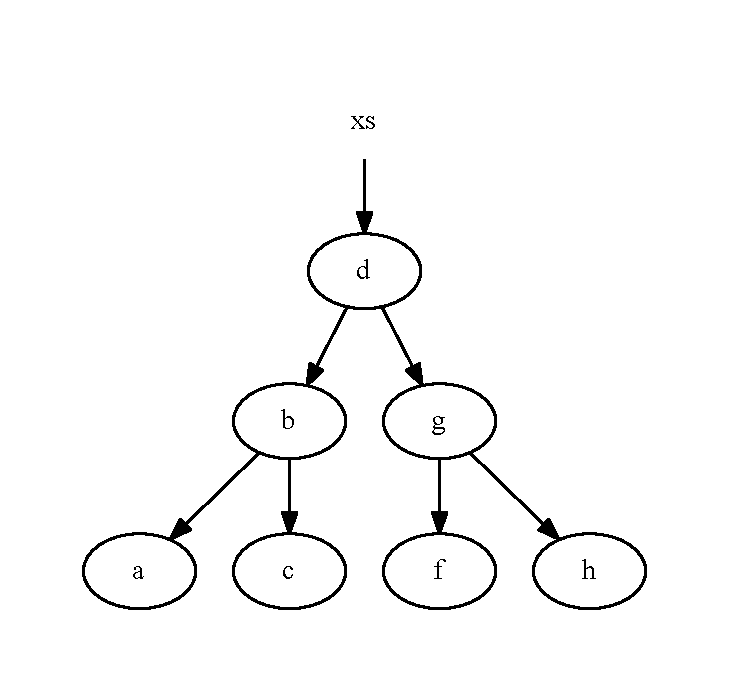
\includegraphics[scale=0.63]{persistent_tree.pdf}  
    \caption{}
  \end{subfigure}
  \begin{subfigure}[b]{0.58\linewidth} 
    \centering
    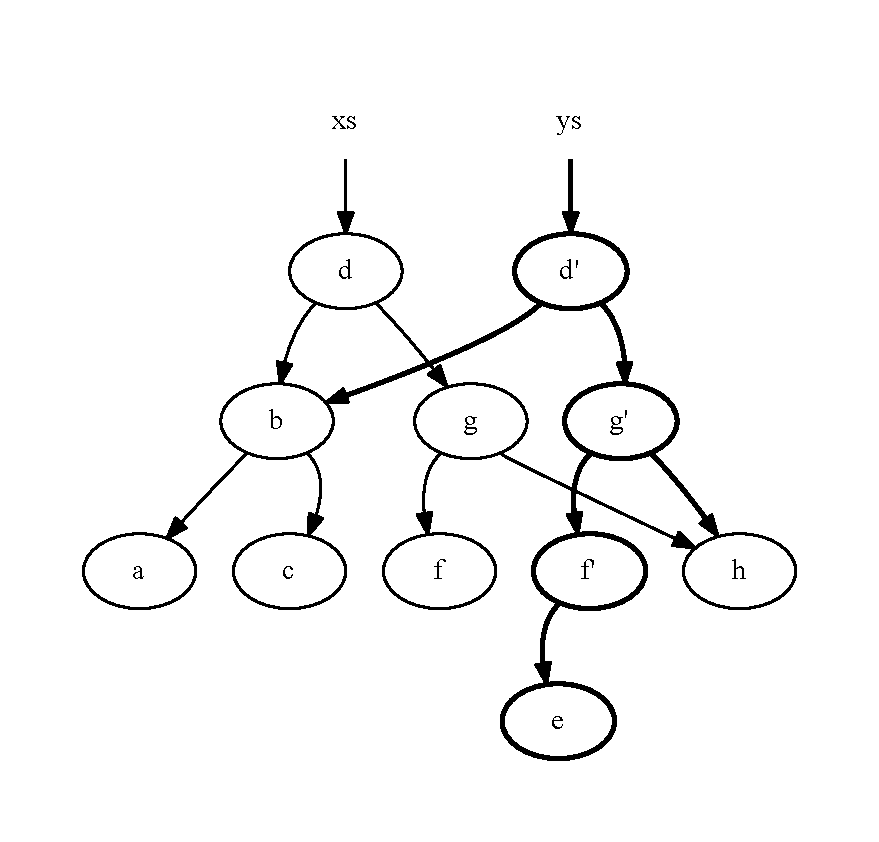
\includegraphics[scale=0.63]{persistent_tree_mod.pdf}  
    \caption{}
  \end{subfigure}
  \caption{ Пример разделения структуры в неизменяемых структурах данных: 
            а "--- исходное дерево;
            б "--- измененное дерево, добавлена вершина \textit{e};}
  \label{fig:arch_and_mod:probab_net:immutable_ds_modification}
\end{figure}

В результате получилось довольно простое и расширяемое представление сети, основное определение которого приведено в листинге~\ref{lst:arch_and_mod:probab_net:bnet_definition}.
Параметризация типа параметрами \lstinline!'NodeAttributes! и \lstinline!'LinkAttributes! и расширяемое устройство типов \lstinline!Node<'T>! и \lstinline!Link<'T>! позволяет достигнуть заявленной расширяемости представления сети и её <<многослойности>>.
Библиотека содержит предопредёленные типы, для представления уровней.
Параметризация типа \lstinline!BNet<unit, unit>! представляет структуру сети и таблицы распределения.
<<Слой>> с дополнительными аттрибутами, планируемыми для использования в алгоритмах статистического вывода суждений представлен типами \lstinline!NodeAttributes<'Annotations>! и \lstinline!LinkAttributes!, но на момент защиты дипломного проекта, из-за неготовой реализации алгоритмов статистического вывода суждений, данные типы содержат не все необходимые атрибуты для работы таких алгоритмов, а лишь прогнозируемых заготовки.
Дополнительный <<слой>>, потенциально необходимый при построении пользовательских приложений, представлен типом \lstinline!VarAnnotations!.
Данный тип содержит дополнительную информацию о переменной, такую как её название и аннотации возможных значений переменной.
Таким образом, наиболее полное представление сети, содержащее все <<слои>>, в коде параметризуется следующим образом \lstinline!BNet<NodeAttributes<VarAnnotations>, LinkAttributes>!.

\begin{lstlisting}[style=fsharpstyle,caption={Определение структуры данных для вероятностной сети}, label=lst:arch_and_mod:probab_net:bnet_definition]
/// Represents immutable BN. Nodes and links between nodes.
type BNet<'NodeAttributes, 'LinkAttributes> = 
    private { nodes: Map<int, Node<'NodeAttributes>>;
              links: Map<int * int, Link<'LinkAttributes>>;
              graph: Graph<int, unit>; } 
\end{lstlisting}

Таким образом, использование параметрического полиморфизма и не\-изменяемых типов данных, позволило добиться поставленных при проектировании целей, а также довольно легкой возможности расширять сеть в дальнейшем.

\subsection{Сохранение сети} % (fold)
\label{sub:arch_and_mod:net_persistence}

Помимо функциональности, связанной с представлением, манипуляцией и выведением структуры сети, разработанная библиотека предоставляет возможность импорта и экспорта вероятностной сети из и в различные форматы.
Т.\,к. библиотека предназначена для работы с модификацией вероятностных сетей, отличающейся в нескольких ключевых моментах от классических байесовых сетей, то нельзя было использовать общепринятые форматы для хранения сетей во внешней памяти и необходимо было разработать свой формат.
Разработанный формат хранения сетей основывается на XML и предназначен для полного сохранения состояния представления сети, используемого в программе.
Данный формат в большей степени похож на ручную сериализацию, чем на удобный формат для обмена вероятностными сетями.
Пример сети, представленной в данном формате, приведен в листинге~\ref{lst:arch_and_mod:net_persistence:bnxml}.

У разработанного формата есть существенный недостаток, его <<понимает>> только разработанная библиотека.
В связи с тем, что в данном дипломном проекте основной целью является реализация лишь малой части возможных операций над вероятностными сетями "--- построение структуры по данным, целесообразно было добавить в библиотеку, хотя и весьма ограниченную, возможность загрузки и сохранения вероятностных сетей из и в существующие распространённые форматы.
Список поддерживаемых форматов приведён в таблице~\ref{table:arch_and_mod:net_persistence:supported_formats}.
Поддержка нескольких форматов понадобилась потому, что многие существующие программы, которые использовались в различной степени для оценки результатов проделанной работы, поддерживают весьма ограниченный набор форматов.
Таким образом, имея возможность экспортировать сеть, построенную одним из алгоритмов реализованных в разработанной библиотеке по данным, в общеиспользуемый формат можно использовать обученную сеть для статистического вывода суждений и других операций в существующих программах, т.\,к. в данный момент в разработанной библиотеке данная функциональность не реализована.
Отдельно стоит отметить возможность сохранения структуры сети в формат представления графов программы GraphViz\footnote{\url{http://www.graphviz.org/}}.
Данное ПО использовалось с целью визуализации выведенных структур и экспорта полученной визуализации в один из векторных графических форматов.
Утилита dot из состава GraphViz умеет автоматически визуализировать сложные графы наилучшим для отображения образом.

\clearpage
\begin{lstlisting}[language=XML,caption={Пример представления простой вероятностной сети в собственном XML"=формате}, label=lst:arch_and_mod:net_persistence:bnxml]
<network>
  <variables>
    <variable id="1" dim="2" />
    <variable id="2" dim="3" />
  </variables>
  <node_attributes>
    <node variable_id="1"> <answered>false</answered> </node>
    <node variable_id="2"> <answered>true</answered>  </node>
  </node_attributes> 
  <link_attributes>
    <link parent_id="1" child_id="2" />
  </link_attributes>
  <variable_annotations>
    <variable_annotation variable_id="1">
      <name>My variable</name>
      <annotations>
        <label>Yes</label> <label>No</label>
      </annotations>
    </variable_annotation>
    <variable_annotation variable_id="2">
      <name>Color</name>
      <annotations>
        <label>Red</label> <label>Green</label> <label>Blue</label>
      </annotations>
    </variable_annotation>
  </variable_annotations>
  <probability_tables>
    <probability_table variable_id="1">
      <vector>0.2 0.8</vector>
    </probability_table>
    <probability_table variable_id="2">
      <vector>0.4 0.3 0.3</vector>
    </probability_table>
  </probability_tables>
  <forward_probability_tables>
    <forward_probability_table variable_id="2" condition_variable_id="1">
      <matrix nrows="3" ncols="2">0.1 0.2 0.7 0.6 0.1 0.3</matrix>
    </forward_probability_table>
  </forward_probability_tables>
</network>
\end{lstlisting}

\begin{table}[ht]
\caption{Поддерживаемые форматы хранения вероятностных сетей}
\label{table:arch_and_mod:net_persistence:supported_formats}
\centering
  \begin{tabular}{| >{\raggedright}m{0.35\textwidth} 
                  | >{\centering}m{0.27\textwidth} 
                  | >{\centering\arraybackslash}m{0.27\textwidth}|}
  \hline Формат & Поддержка импорта & Поддержка экспорта \\
  \hline Собственный xml"=формат & полная & полная \\
  \hline XMLBIF & частичная & частичная \\
  \hline GeNIe & частичная & отсутствует \\
  \hline GraphViz dot & отсутствует & полная \\
  \hline
  \end{tabular}
\end{table}



\subsection{Представление экспериментальных данных}
\label{sub:arch_and_mod:dataframe}

Немаловажной задачей в обучении и построении структуры сети по данным является представление набора экспериментальных данных в оперативной и постоянной памяти.
В машинном обучении и других областях, связанных с обработкой массивов данных, для хранения данных на диске в большинстве случаев применяется простой текстовый формат \emph{csv} "--- значения, разделённые специальным символом и записанные в текстовый файл построчно.
В разработанной библиотеке также используется данный формат для импортирования экспериментальных данных с диска в память программы для дальнейшей обработки.
Для чтения \emph{csv} файлов используется легковесная внешняя библиотека LumenWorks.Framework.IO\footnote{\url{http://www.codeproject.com/Articles/9258/A-Fast-CSV-Reader}}.

Для представления набора экспериментальны данных в библиотеке присутствует специальный тип "--- DataFrame, который представляет из себя информацию о переменных и, собственно, набор экспериментальных данных в компактном для хранения виде.
Из особенностей реализации стоит упомянуть способ достижения компактности хранения.
При чтении \emph{csv} файла каждому состоянию переменной назначается некоторое 8-битное число, которое является представлением данного состояния в памяти компьютера.
Использование 8"=битного числа с одной стороны ограничивает число возможных состояний одной переменной до \num{256}, с другой стороны "--- данное представление достаточно компактно, чтобы быть пригодным для работы на персональном компьютере разработчика с ограниченным размером ОЗУ и уметь обрабатывать наборы данных из миллионов случаев для десятков переменных.
Одной из дополнительных возможностей DataFrame является возможность производить случайные выборки из имеющегося набора данных.
Данная возможность была использована при реализации алгоритмов вывода структуры вероятностной сети по данным.


\subsection{Байесовы сети Asia и ALARM}
\label{sub:arch_and_mod:asia_and_alarm}

Перед тем как перейти к обсуждению разработанных алгоритмов вывода структуры сети по данным целесообразно обсудить известные сети, которые использовались в качестве моделей для вывода по экспериментальным данным.
Речь пойдет о ставших уже классикой в таких задачах "--- сетях Asia и ALARM.

\subsubsection{Asia }
\label{sub:arch_and_mod:asia_and_alarm:asia}

Байесова сеть Asia является небольшой синтетической сетью, обычно используемой при изучении вероятностных сетей.
Данная вероятностная сеть рассмотрена в работе~\cite{Lauritzen_Spiegelhalter88}.
Искусственная байеосова сеть Asia предназначена для диагностики у пациентов заболеваний связанных с лёгкими.
В перечень диагностируемых болезней входят туберкулёз, рак и бронхит.
Данная сеть имеет восемь бинарных случайных величин.
Структура данной сети приведена на рисунке~\ref{fig:domain:programs:our_impl_plus_asia}~(б) на странице~\pageref{fig:domain:programs:our_impl_plus_asia}.
В таблице~\ref{table:arch_and_mod:asia_and_alarm:asia:vars} приведено описание переменных.

\begin{table}[ht]
\caption{Описание переменных сети Asia}
\label{table:arch_and_mod:asia_and_alarm:asia:vars}
\centering
  \begin{tabular}{| >{\raggedright}m{0.17\textwidth} 
                  | >{\centering}m{0.17\textwidth} 
                  | >{\raggedright\arraybackslash}m{0.57\textwidth}|}
  \hline Переменная & Количество состояний & \begin{center} Примечание \end{center} \\
  \hline VisitAsia & \num{2} & посещал ли пациент Азию \\
  \hline Tuberculosis & \num{2} & болен туберкулёзом \\
  \hline Smoking & \num{2} & курит \\
  \hline Cancer & \num{2} & имеет рак легких \\
  \hline TbOrCa & \num{2} & имеет рак или туберкулёз \\
  \hline XRay & \num{2} & плохая рентгенография \\
  \hline Bronchitis & \num{2} & болен бронхитом \\
  \hline Dyspnea & \num{2} & испытывает удушье \\
  \hline
  \end{tabular}
\end{table}


\subsubsection{ALARM }
\label{sub:arch_and_mod:asia_and_alarm:alarm}

Данная байесова сеть также очень часто рассматривается для оценки качества различных алгоритмов, работающих с вероятностными сетями.
Данная сеть была рассмотрена в работе~\cite{beinlich1989alarm}.
Сеть предназначена для медицинской диагностики, и используется для обработки физиологических наблюдений пациента.
Сеть состоит из переменных трех типов: диагнозов, физиологических показателей и скрытых переменных, которые измерить на практике нельзя.
Данная сеть содержит \num{37} переменных и \num{46} связей между ними.
Максимальное количество переменных"=родителей равно четырём.
Рассматриваемая вероятностная сеть относится к сетям средник размеров.
Данная сеть хорошо изучена и представляет интерес, как модель для оценки качества реализованных в библиотеке алгоритмов.
Структура сети приведена на рисунке~\ref{fig:arch_and_mod:asia_and_alarm:alarm_structure}.
Из-за довольно большого количества переменных здесь не приводится их описание и назначение.
В этой информации нет необходимости для оценки качества реализованных алгоритмов, важно знать общую структуру сети.

\begin{figure}[ht!]
  \hspace{-4ex} % Кривой хак чтобы подвинуть картинку к левому краю страницы
  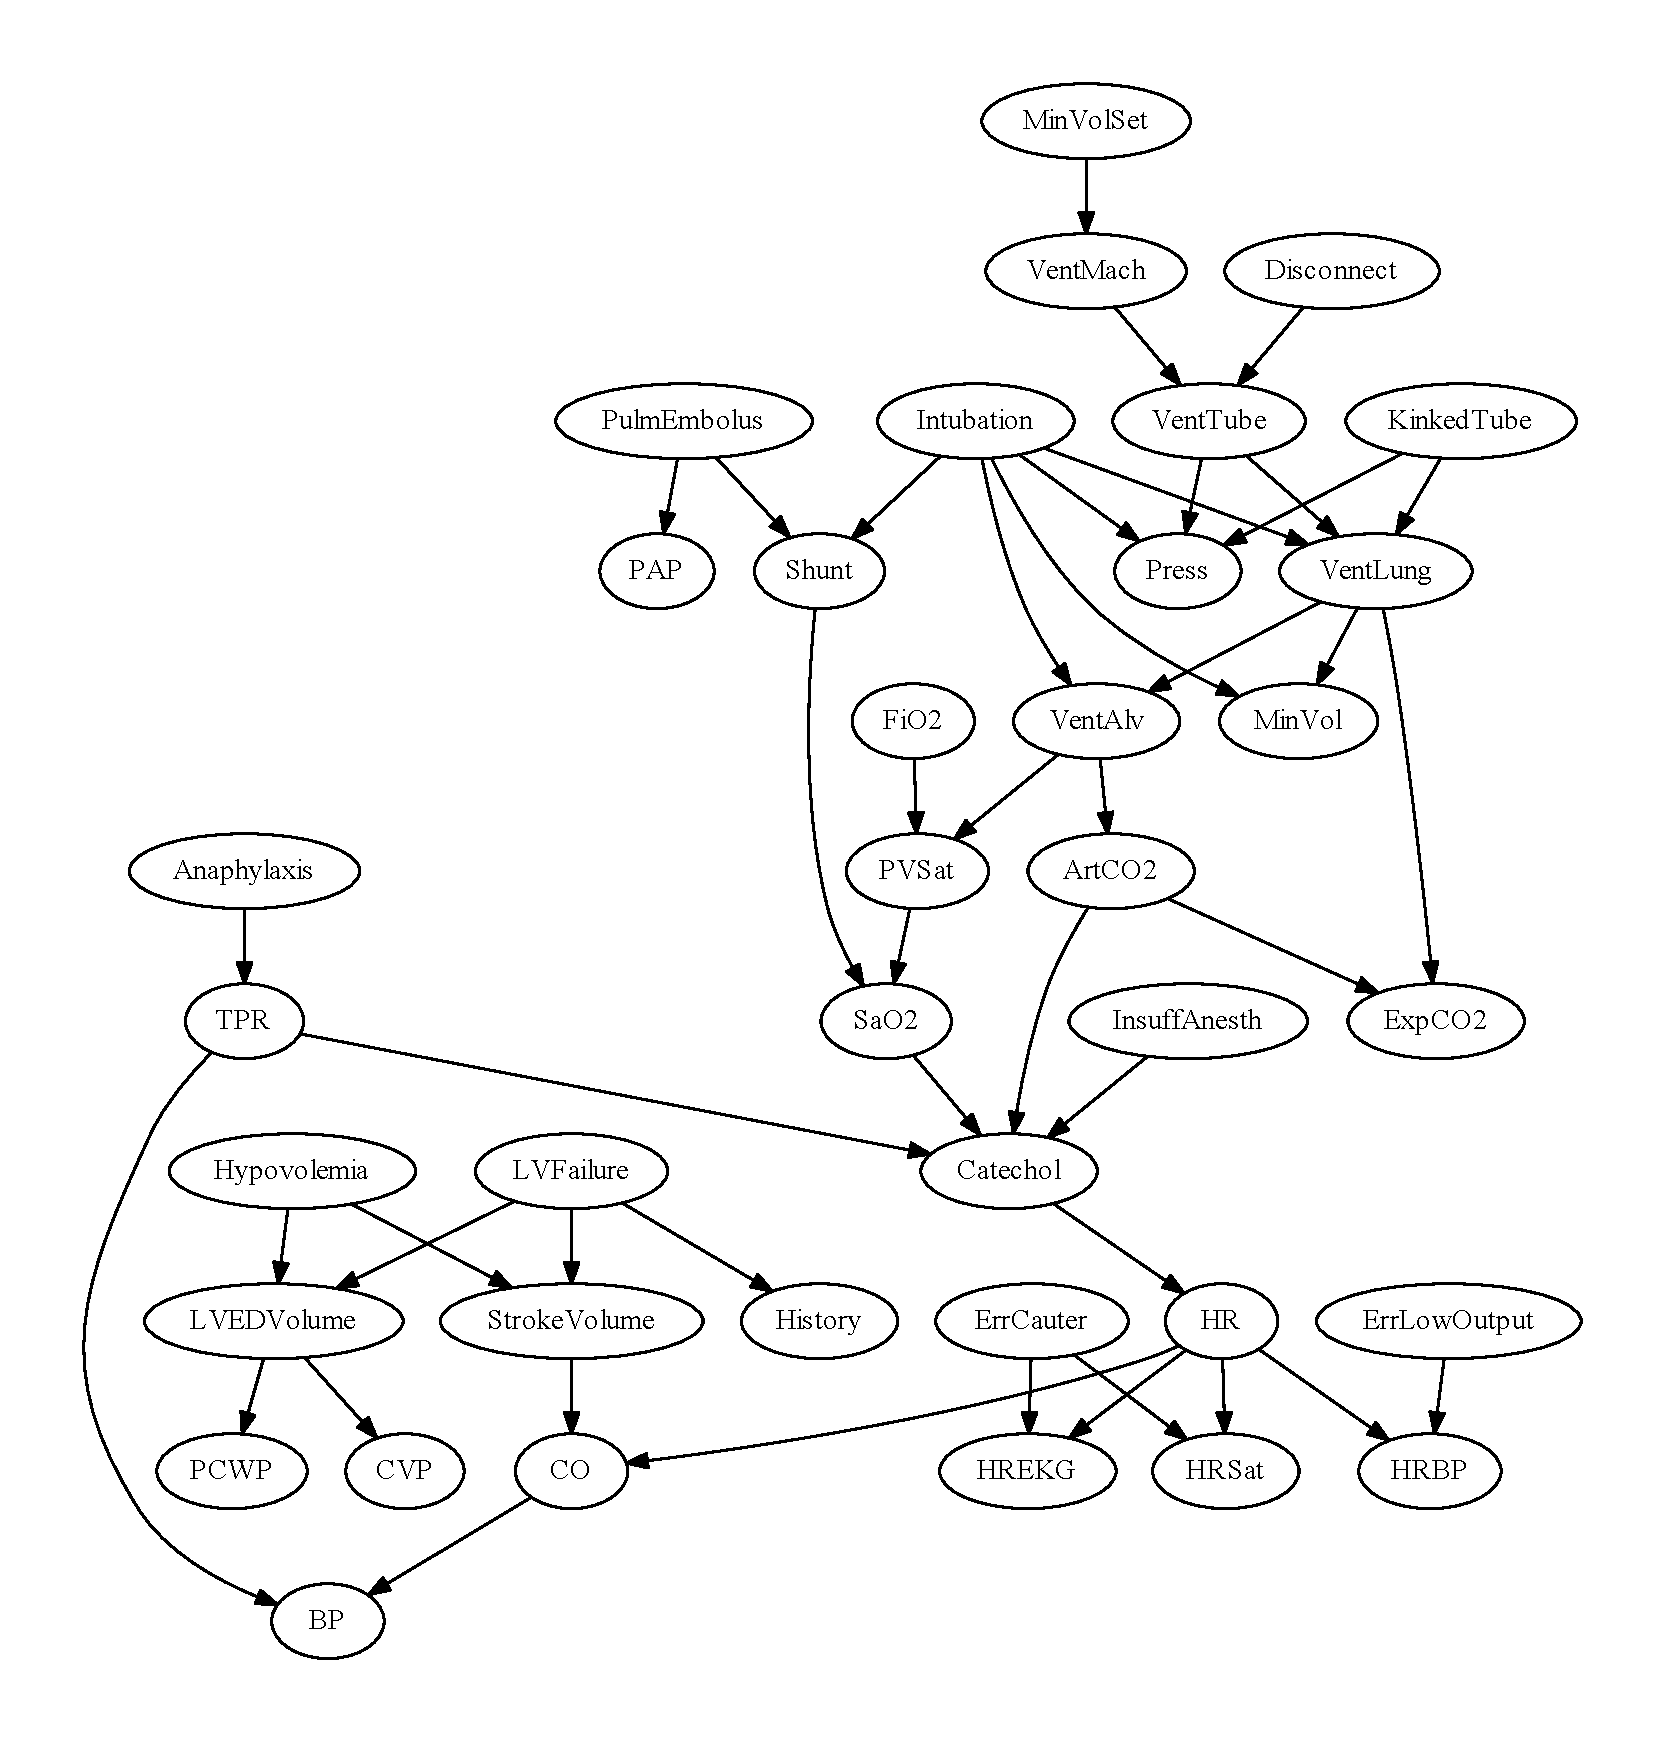
\includegraphics[scale=0.6]{alarm_reference_net.pdf}  
  \caption{ Структура байесовой сети ALARM }
  \label{fig:arch_and_mod:asia_and_alarm:alarm_structure}
\end{figure}


\subsection{Алгоритм на основе оценки апостериорной вероятности структуры}
\label{sub:arch_and_mod:k2_algorithm}

В данном подразделе рассматривается известный алгоритм, использующий оценку апостериорной вероятности в качестве критерия поиска.
Подробное описание данной оценки и базового алгоритма поиска приведены в работе~\cite{Cooper1991}. 

Формулу~(\ref{eq:domain:k2:model_and_data_prob}) для оценки совместной вероятности на практике напрямую использовать не получится, без введения дополнительных предположений.
Необходимо сделать предположение, что все возможные структуры равновероятны, т.\,е. $P(B_S)$ равно некоторой малой константе $c$.
Таким образом нахождение оптимальной структуры сводится к максимизации формулы~(\ref{eq:arch_and_mod:k2_algorithm:optimization_objective}), т.\,e. задача сводится к нахождению множества вершин"=предков $ \pi_i $ для каждой вершины $X_i$, оптимизирующих целевую функцию~\cite{Cooper1991}.
\begin{align}
  \label{eq:arch_and_mod:k2_algorithm:optimization_objective}
  \max \left[ P(B_S, x^R[n]) \right] = \notag\\
  =
    c \prod_{i = 1}^{R} \max_{\pi_i} 
    \bigg[
      \prod_{j = 1}^{q_i} &% to align formula
      \frac{(\alpha_i - 1)!}
           {(n[\phi_i[j], i, B_S] + \alpha_i - 1)!}
      \prod_{k = 1}^{\alpha_i}
        n[v_{ik}, \phi_i[j], i, B_S]! 
    \bigg] \text{\,.}
\end{align}

Таким образом наивный алгоритм поиска состоит в полном переборе всех возможных родителей для каждой вершины и оптимизации при этом функции~(\ref{eq:arch_and_mod:k2_algorithm:node_optimization_obj}):
\begin{equation}
  \label{eq:arch_and_mod:k2_algorithm:node_optimization_obj}
  g(i, \pi_i) =       
    \prod_{j = 1}^{q_i}
      \frac{(\alpha_i - 1)!}
           {(n[\phi_i[j], i, B_S] + \alpha_i - 1)!}
      \prod_{k = 1}^{\alpha_i}
        n[v_{ik}, \phi_i[j], i, B_S]! \text{\,.}
\end{equation}

На практике наивный вариант не годится из-за большого количества возможных вариантов структур сетей.
В разработанной реализации использовались те же ограничения и стратегия поиска, что и в работе~\cite{Cooper1991}.
Перед началом выполнения алгоритма требуется знание о порядке вершин, таком, что вершины родители всегда находятся раньше вершин потомков.
Схематически алгоритм поиска выглядит следующим образом:

\begin{lstlisting}[mathescape,escapeinside={/*@}{@*/},caption={Псевдокод реализации алгоритма К2}, label=lst:arch_and_mod:k2_algorithm:k2_pseudo]
function k2 =
  (* Input: dataset $x^R[n]$, ordering of variables, u - maximum number of parents per variable.
     Output: for each node, a printout of the parents of the node. *)
  for i in 1 .. R do
    $ \pi_i $ := $ \emptyset $
    $P_{old}$ := $g(i, \pi_i)$; // formula(/*@\ref{eq:arch_and_mod:k2_algorithm:node_optimization_obj}@*/)
    OkToContinue := true;
    while OkToContinue and $|\pi_i| < u$ do
      let z = node in $ \text{Pred}(X_i) - \pi_i $ that maximizes $ g(i, \pi_i \cup {z}) $
      $P_{new}$ := $f(i, \pi_i \cup {z})$
      if $P_{new} > P_{old}$ then
        $P_{old}$ := $P_{new}$;
        $ \pi_i $ := $ \pi_i \cup {z} $
      else OkToContinue := false
    end while
    printfn("Node: ", $X_i$, "Parents of $X_i$:", $\pi_i$)
  end for
end
\end{lstlisting}

В разработанной в рамках дипломного проекта реализации за основу был взят алгоритм К2, приведенный в работе~\cite{Cooper1991}, псевдокод которого показан в листинге~\ref{lst:arch_and_mod:k2_algorithm:k2_pseudo}.
В разработанном алгоритме слегка изменен способ подсчета целевой функции.
Приняв во внимание ограничение на представление в компьютере вещественных и больших целых чисел, а также то, что операции умножения, деления и возведения в степень более сложные, было принято решение воспользоваться прологарифмированной версией формулы~(\ref{eq:arch_and_mod:k2_algorithm:node_optimization_obj}).
Ниже приводится точная формула~(\ref{eq:arch_and_mod:k2_algorithm:log_node_optimization_obj}), по которой вычисляется оценка в реализованном алгоритме.
Данная формула более удобная для вычисления на компьютере:

\begin{align}
  \label{eq:arch_and_mod:k2_algorithm:log_node_optimization_obj}
  \log(g(i, \pi_i)) &=
    \sum_{j = 1}^{q_i}
      \log 
      \left(
        \frac{(\alpha_i - 1)!}
             {(n_{ij} + \alpha_{i} - 1)!}
        \prod_{k = 1}^{\alpha_i}
          n_{ijk}!
      \right) =\notag\\
    &=
    \sum_{j = 1}^{q_i}
      \left(
        \log
          \frac{(\alpha_i - 1)!}
               {(n_{ij} + \alpha_{i} - 1)!}
        +
        \log 
          \prod_{k = 1}^{\alpha_i}
            n_{ijk}!
      \right) =\notag\\
    &=
    \sum_{j = 1}^{q_i}
      \left(
        \log (\alpha_i - 1)! - \log (n_{ij} + \alpha_{i} - 1)!
        +
        \sum_{k = 1}^{\alpha_i}
          \log n_{ijk}!
      \right) =\notag\\
    &=
      \sum_{j = 1}^{q_i}
      \left(
        \log \Gamma(\alpha_i) - \log \Gamma(n_{ij} + \alpha_{i})
        +
        \sum_{k = 1}^{\alpha_i}
          \log \Gamma(n_{ijk} + 1)
      \right) = \notag\\
    &=
      q_i \log \Gamma(\alpha_i) +
      \sum_{j = 1}^{q_i}
      \left(
        \sum_{k = 1}^{\alpha_i}
          \log \Gamma(n_{ijk} + 1)
        - \log \Gamma(n_{ij} + \alpha_{i})
      \right) \text{\,,}
\end{align}
\begin{explanation}
где & $ \Gamma $ & гамма-функция "---  расширение понятия факториала на поле комплексных чисел; \\
    & $ n_{ijk} $ & условное, более краткое, обозначение для $n[v_{ik}, \phi_i[j], i, B_S]$; \\
    & $ n_{ij} $ & условное, более краткое, обозначение для $n[\phi_i[j], i, B_S]$. 
\end{explanation}

Помимо использования формулы~(\ref{eq:arch_and_mod:k2_algorithm:log_node_optimization_obj}) в реализации были произведены дополнительные оптимизации, продиктованные результатами профилирования реализации алгоритма.

Результаты обучения сетей Asia и ALARM на наборах данных разного объёма реализованным алгоритмом приведены в таблицах~\ref{table:arch_and_mod:k2_algorithm:result_asia} и~\ref{table:arch_and_mod:k2_algorithm:result_alarm} соответственно\footnote{Формат времени в колонке <<Время построения>> "--- часы:минуты:секунды.милисекунды}.
Как видно из результатов, с увеличением количества данных улучшается качество извлеченной из данных сети.
Стоит обратить внимание, что данный алгоритм потребовал априорных знаний о распределении, по которому были сгенерированы данные.
Алгоритму на вход необходим определенный порядок вершин и знание максимального количества переменных"=родителей для каждой переменной.

\begin{table}[ht]
\caption{Качество структуры извлеченной из данных для сети Asia алгоритмом К2 из разработанной библиотеки}
\label{table:arch_and_mod:k2_algorithm:result_asia}
  \centering
  \begin{tabular}{| >{\raggedleft}m{0.14\textwidth} 
                  | >{\centering}m{0.15\textwidth} 
                  | >{\centering}m{0.15\textwidth} 
                  | >{\centering}m{0.195\textwidth} 
                  | >{\centering\arraybackslash}m{0.23\textwidth}|}
    \hline
    \multirow{2}{0.14\textwidth}{\centering Размер данных} &
    \multicolumn{3}{c|}{\centering Соединения} &
    \multirow{2}{0.22\textwidth}{\centering Время построения} \\
    \cline{2-4}
    & пропущено & добавлено & инвертировано & \\
    \hline
     \num{1000} & \num{1} & \num{1} & \num{0} & 00:00:00.01 \\
    \hline
     \num{2000} & \num{1} & \num{1} & \num{0} & 00:00:00.02 \\
    \hline
     \num{4000} & \num{1} & \num{0} & \num{0} & 00:00:00.04 \\
    \hline
     \num{8000} & \num{1} & \num{1} & \num{0} & 00:00:00.09 \\
    \hline
     \num{16000} & \num{0} & \num{0} & \num{0} & 00:00:00.17 \\
    \hline
     \num{32000} & \num{0} & \num{0} & \num{0} & 00:00:00.36 \\
    \hline
     \num{64000} & \num{0} & \num{0} & \num{0} & 00:00:00.80 \\
    \hline
     \num{1048576} & \num{0} & \num{0} & \num{0} & 00:00:11.41 \\
    \hline
  \end{tabular}
\end{table}

\begin{table}[ht]
\caption{Качество структуры извлеченной из данных для сети ALARM алгоритмом К2 из разработанной библиотеки}
\label{table:arch_and_mod:k2_algorithm:result_alarm}
  \centering
  \begin{tabular}{| >{\raggedleft}m{0.14\textwidth} 
                  | >{\centering}m{0.15\textwidth} 
                  | >{\centering}m{0.15\textwidth} 
                  | >{\centering}m{0.195\textwidth} 
                  | >{\centering\arraybackslash}m{0.23\textwidth}|}
    \hline
    \multirow{2}{0.14\textwidth}{\centering Размер данных} &
    \multicolumn{3}{c|}{\centering Соединения} &
    \multirow{2}{0.22\textwidth}{\centering Время построения} \\
    \cline{2-4}
    & пропущено & добавлено & инвертировано & \\
    \hline
     \num{1000} & \num{1} & \num{5} & \num{0} & 00:00:00.75 \\
    \hline
     \num{2000} & \num{1} & \num{1} & \num{0} & 00:00:00.72 \\
    \hline
     \num{4000} & \num{1} & \num{0} & \num{0} & 00:00:01.29 \\
    \hline
     \num{8000} & \num{1} & \num{2} & \num{0} & 00:00:02.45 \\
    \hline
     \num{16000} & \num{0} & \num{2} & \num{0} & 00:00:04.83 \\
    \hline
     \num{32000} & \num{0} & \num{1} & \num{0} & 00:00:09.48 \\
    \hline
     \num{64000} & \num{0} & \num{1} & \num{0} & 00:00:18.61 \\
    \hline
     \num{128000} & \num{0} & \num{1} & \num{0} & 00:00:36.58 \\
    \hline
     \num{1048576} & \num{0} & \num{1} & \num{0} & 00:04:57.18 \\
    \hline
     \num{8388608} & \num{0} & \num{1} & \num{0} & 00:44:13.00 \\
    \hline
  \end{tabular}
\end{table}

Произведём сравнение реализованного алгоритма, с аналогичным алгоритмом реализованным в программе GeNIe, описанной в пункте~\ref{sub:domain:existing_programs:genie} на странице~\pageref{sub:domain:existing_programs:genie}.
В таблице~\ref{table:arch_and_mod:k2_algorithm:genie_asia_k2} приводятся полученные результаты.

\begin{table}[ht]
\caption{Качество структуры извлеченной из данных для сети Asia программой GeNIe с применением алгоритма Greedy Thick Thinning с оценкой K2}
\label{table:arch_and_mod:k2_algorithm:genie_asia_k2}
  \centering
  \begin{tabular}{| >{\raggedleft}m{0.14\textwidth} 
                  | >{\centering}m{0.15\textwidth} 
                  | >{\centering}m{0.15\textwidth} 
                  | >{\centering}m{0.195\textwidth} 
                  | >{\centering\arraybackslash}m{0.23\textwidth}|}
    \hline
    \multirow{2}{0.14\textwidth}{\centering Размер данных} &
    \multicolumn{3}{c|}{\centering Соединения} &
    \multirow{2}{0.22\textwidth}{\centering Время построения} \\
    \cline{2-4}
    & пропущено & добавлено & инвертировано & \\
    \hline
     \num{1000} & \num{2} & \num{2} & \num{2} & \emph{не измерялось} \\
    \hline
     \num{2000} & \num{2} & \num{3} & \num{2} & \emph{не измерялось} \\
    \hline
     \num{4000} & \num{1} & \num{1} & \num{3} & \emph{не измерялось} \\
    \hline
     \num{8000} & \num{2} & \num{4} & \num{2} & \emph{не измерялось} \\
    \hline
     \num{16000} & \num{2} & \num{5} & \num{2} & \emph{не измерялось} \\
    \hline
     \num{32000} & \num{1} & \num{4} & \num{2} & \emph{не измерялось} \\
    \hline
     \num{64000} & \num{0} & \num{1} & \num{3} & \emph{не измерялось} \\
    \hline
     \num{1048576} & \num{1} & \num{4} & \num{2} & \emph{не измерялось} \\
    \hline
  \end{tabular}
\end{table}

Для сравнения реализованных в библиотеке алгоритмов с теми, которые есть в GeNIe, были произведены дополнительные испытания последних.
Для наиболее <<точного>> алгоритма реализованного в GeNIe в таблице~\ref{table:arch_and_mod:k2_algorithm:genie_asia_pc} приводится оценка качества полученной структуры на наборах данных различного размера
Для трех других алгоритмов в таблице~\ref{table:arch_and_mod:k2_algorithm:genie_asia_other} "--- на самом большом наборе данных.
Как видно из полученных экспериментально данных, реализация алгоритма на основе оценки апостериорной вероятности из разработанной библиотеки ведет себя лучше как на малых объёмах данных, так и на больших, не смотря на то, что некоторые алгоритмы реализованные в GeNIe используют тот же метод оценки.

\begin{table}[ht]
\caption{Качество структуры извлеченной из данных для сети Asia программой GeNIe с использованием алгоритма PC}
\label{table:arch_and_mod:k2_algorithm:genie_asia_pc}
  \centering
  \begin{tabular}{| >{\raggedleft}m{0.14\textwidth} 
                  | >{\centering}m{0.15\textwidth} 
                  | >{\centering}m{0.15\textwidth} 
                  | >{\centering}m{0.195\textwidth} 
                  | >{\centering\arraybackslash}m{0.23\textwidth}|}
    \hline
    \multirow{2}{0.14\textwidth}{\centering Размер данных} &
    \multicolumn{3}{c|}{\centering Соединения} &
    \multirow{2}{0.22\textwidth}{\centering Время построения} \\
    \cline{2-4}
    & пропущено & добавлено & инвертировано & \\
    \hline
     \num{1000} & \num{2} & \num{1} & \num{2} & \emph{не измерялось} \\
    \hline
     \num{2000} & \num{3} & \num{0} & \num{0} & \emph{не измерялось} \\
    \hline
     \num{4000} & \num{1} & \num{0} & \num{0} & \emph{не измерялось} \\
    \hline
     \num{8000} & \num{2} & \num{0} & \num{0} & \emph{не измерялось} \\
    \hline
     \num{16000} & \num{3} & \num{1} & \num{3} & \emph{не измерялось} \\
    \hline
     \num{32000} & \num{2} & \num{0} & \num{0} & \emph{не измерялось} \\
    \hline
     \num{64000} & \num{1} & \num{0} & \num{0} & \emph{не измерялось} \\
    \hline
     \num{1048576} & \num{1} & \num{0} & \num{0} & \emph{не измерялось} \\
    \hline
  \end{tabular}
\end{table}

\begin{table}[ht]
\caption{Качество структуры извлеченной из данных для сети Asia программой GeNIe на наборе данных из \num{1048576} случаев}
  \label{table:arch_and_mod:k2_algorithm:genie_asia_other}
  \centering
  \begin{tabular}{| >{\raggedright}m{0.405\textwidth} 
                  | >{\centering}m{0.15\textwidth} 
                  | >{\centering}m{0.14\textwidth} 
                  | >{\centering\arraybackslash}m{0.195\textwidth}|}
    \hline
    \multirow{2}{0.37\textwidth}{\centering Алгоритм} &
    \multicolumn{3}{c|}{\centering Соединения}  \\
    \cline{2-4}
    & пропущено & добавлено & инвертировано \\
    \hline
     Bayesian Search & \num{0} & \num{2} & \num{5} \\
    \hline
     Essential Graph Search & \num{5} & \num{0} & \num{2} \\
    \hline
     Greedy Thick Thinning с оценкой BDeu & \num{1} & \num{4} & \num{2} \\
    \hline
  \end{tabular}
\end{table}


\subsection{Алгоритм на основе оценки минимальной длины описания}
\label{sub:arch_and_mod:mdl_algorithm1}
Помимо алгоритма использующего оценку апостериорной вероятности в разработанной библиотеке был реализован алгоритм использующий оценку на основе принципа МДО.
Описание принципа МДО приведено в подразделе~\ref{sub:domain:mdl_principle} данной пояснительной записки.
Т.\,к. способ подсчета оценки уже был здесь описан, то необходимо привести описание процедуры поиска.
Процедура поиска в разработанной реализации алгоритма поиска вдохновлена процедурой поиска, использованной в работе~\cite{terentyev_2006}.

Данный алгоритм нахождения структуры не требует предварительных знаний об истинном распределении, в отличие от алгоритма описанного в подразделе~\ref{sub:arch_and_mod:k2_algorithm}, что является существенным преимуществом на практике.
Вместо использования априорных знаний, реализация алгоритма используем предварительные вычисления, извлекающие полезные данные о взаимозависимостях между переменным.
Затем эта информация используется в стратегии поиска структуры.

В качестве оценки степени зависимости двух произвольных переменных в работе~\cite{Chow68approximatingdiscrete} было предложено использовать значение взаимной информации\footnote{В англоязычной литературе используется термин mutual information}.
Эта информация задаёт приоритет поиска зависимостей между переменными.
По своей сути значение обоюдной информации является аналогом корреляции, но по своему содержанию "--- это оценка количества информации содержащейся в одной переменной о другой~\cite{terentyev_2006}.
Значение взаимной информации принимает неотрицательные значения и равно нулю в случае независимости случайных величин.
Для вычисления взаимной информации была предложена формула~(\ref{eq:arch_and_mod:mdl_algorithm1:mutual_information}):
\begin{equation}
  \label{eq:arch_and_mod:mdl_algorithm1:mutual_information}
  I(X; Y) = \sum_{y \in Y} \sum_{x \in X} 
                 p(x, y) \log{ \left(\frac{p(x, y)}{p(x)\,p(y)}
                              \right) } \text{\,,}
\end{equation}
\begin{explanation}
где & $ p(x, y)$ & совместное распределение случайных величин $X$ и $Y$; \\
    & $ p(y) $ & безусловное распределение случайной величины $X$; \\
    & $ p(x) $ & безусловное распределение случайной величины $Y$.
\end{explanation}

На практике при вычислении $I(X; Y)$ следует соблюдать осторожность, т.\,к. относительные частоты, используемые для оценки $p(x)$, $p(y)$ и $p(x, y)$, могут необоснованно принимать значение \num{0} из-за отсутствия некоторых состояний переменных в наблюдаемых данных.
В таких случаях вместо нуля используется достаточно малое число.

Таким образом алгоритм поиска состоит из следующих шагов:
\begin{enumerate}
  \item Вычислить значения взаимной информации между всеми парами переменных и отсортировать список уникальных пар по убыванию взаимной информации.
  Пусть данный список обозначается символом $list$.
  \item Алгоритм поиска начинается с извлечения двух пар переменных $(X_{i1}, X_{i2})$ и $(X_{j1}, X_{j2})$ из списка $list$ с максимальным значением взаимной информации.
  Затем среди всех возможных ацикличных моделей, построенных из переменных $ X_{i1}, X_{i2}, X_{j1}, X_{j2} $ выбирается модель с наименьшей оценкой, вычисленной по формуле~(\ref{eq:domain:mdl:description_length}).
  Эта модель принимается за стартовую модель $g_0$
  \item Пока список $list$ не пуст из него извлекается пара переменных $(X_{k1}, X_{k2})$ и строится множество новых моделей $\{g_0; g_0 \cup (X_{k1}, X_{k2}); g_0 \cup (X_{k2}, X_{k1})\} $.
  И этого множества удаляются циклические модели и выбирается модель с минимальной оценкой по формуле~(\ref{eq:domain:mdl:description_length}) и присваивается переменной $g_0$.
  \item Когда список $list$ пуст, то поиск прекращается, модель $g_0$ считается оптимальной и рассматривается как структура вероятностной сети выведенная из данных. 
  На практике можно завершить алгоритм раньше не дожидаясь пустоты $list$.
\end{enumerate}

При реализации данного алгоритма важным моментом для повышения производительности является мемоизация значений функций $n[s, k, g]$ и $n[q, s, k, g]$, т.\,к. оценка длины описания считается для всей модели сразу, но между двумя последовательными итерациями разница между моделями составляем максимум одно соединение, т.\,е. для большинства вершин множество предков не меняется и значения $n[s, k, g]$ и $n[q, s, k, g]$ остаются неизменными и их можно не вычислять каждый раз.
Так, для сети ALARM на экспериментальных данных из \num{1048576} случаев, время построения сети сократилось с более чем четырех часов, до двух с половиной минут.
Ниже приведены результаты качества обучения данного алгоритма для сети Asia, в табилце~\ref{table:arch_and_mod:mdl_algorithm1:asia_mdl}, и для сети ALARM, в таблице~\ref{table:arch_and_mod:mdl_algorithm1:alarm_mdl}.

\begin{table}[ht]
\caption{Качество структуры извлеченной из данных для сети Asia алгоритмом из разработанной библиотеки, использующим оценку МДО}
\label{table:arch_and_mod:mdl_algorithm1:asia_mdl}
  \centering
  \begin{tabular}{| >{\raggedleft}m{0.14\textwidth} 
                  | >{\centering}m{0.15\textwidth} 
                  | >{\centering}m{0.15\textwidth} 
                  | >{\centering}m{0.195\textwidth} 
                  | >{\centering\arraybackslash}m{0.23\textwidth}|}
    \hline
    \multirow{2}{0.14\textwidth}{\centering Размер данных} &
    \multicolumn{3}{c|}{\centering Соединения} &
    \multirow{2}{0.22\textwidth}{\centering Время построения} \\
    \cline{2-4}
    & пропущено & добавлено & инвертировано & \\
    \hline
     \num{1000} & \num{2} & \num{1} & \num{0} & 00:00:00.26 \\
    \hline
     \num{2000} & \num{2} & \num{2} & \num{2} & 00:00:00.28 \\
    \hline
     \num{4000} & \num{1} & \num{2} & \num{2} & 00:00:00.47 \\
    \hline
     \num{8000} & \num{1} & \num{1} & \num{0} & 00:00:00.93 \\
    \hline
     \num{16000} & \num{1} & \num{2} & \num{0} & 00:00:01.70 \\
    \hline
     \num{32000} & \num{0} & \num{1} & \num{1} & 00:00:03.37 \\
    \hline
     \num{64000} & \num{0} & \num{1} & \num{0} & 00:00:07.05 \\
    \hline
     \num{1048576} & \num{0} & \num{1} & \num{0} & 00:01:46.53 \\
    \hline
  \end{tabular}
\end{table}

\begin{table}[ht]
\caption{Качество структуры извлеченной из данных для сети ALARM алгоритмом из разработанной библиотеки, использующим оценку МДО}
\label{table:arch_and_mod:mdl_algorithm1:alarm_mdl}
  \centering
  \begin{tabular}{| >{\raggedleft}m{0.14\textwidth} 
                  | >{\centering}m{0.15\textwidth} 
                  | >{\centering}m{0.15\textwidth} 
                  | >{\centering}m{0.195\textwidth} 
                  | >{\centering\arraybackslash}m{0.23\textwidth}|}
    \hline
    \multirow{2}{0.14\textwidth}{\centering Размер данных} &
    \multicolumn{3}{c|}{\centering Соединения} &
    \multirow{2}{0.22\textwidth}{\centering Время построения} \\
    \cline{2-4}
    & пропущено & добавлено & инвертировано & \\
    \hline
     \num{1000} & \num{6} & \num{3} & \num{11} & 00:00:01.78 \\
    \hline
     \num{2000} & \num{5} & \num{5} & \num{11} & 00:00:01.50 \\
    \hline
     \num{4000} & \num{3} & \num{4} & \num{11} & 00:00:01.84 \\
    \hline
     \num{8000} & \num{3} & \num{7} & \num{9} & 00:00:02.26 \\
    \hline
     \num{16000} & \num{2} & \num{10} & \num{17} & 00:00:03.27 \\
    \hline
     \num{32000} & \num{2} & \num{13} & \num{19} & 00:00:05.17 \\
    \hline
     \num{64000} & \num{1} & \num{17} & \num{15} & 00:00:09.30 \\
    \hline
     \num{128000} & \num{1} & \num{21} & \num{21} & 00:00:18.50 \\
    \hline
     \num{1048576} & \num{0} & \num{22} & \num{16} & 00:02:22.82 \\
    \hline
  \end{tabular}
\end{table}

Как видно данный алгоритм работает хуже алгоритма из подраздела~\ref{sub:arch_and_mod:k2_algorithm}.
По результатам измерений, приведенных в табилце~\ref{table:arch_and_mod:mdl_algorithm1:alarm_mdl} можно видеть, что с увеличением набора данных структура сети усложняется.
Количество пропущенных связей уменьшается, но также растет количество лишних и инвертированных связей.
На практике возможна доработка структуры сети с участием эксперта.
Это займет меньше времени, чем разработка сети <<с нуля>>, т.\,к. большинство связей и общая структура уже найдены.
В защиту данного алгоритма можно сказать, что он работает без каких-либо априорных знаний о структуре сети и не ограничен максимальным количеством вершин"=предков, как алгоритм из предыдущего подраздела.
Также можно заметить, что не смотря на то, что алгоритм проигрывает реализации алгоритма K2, качество обучаемой структуры в многих случаях лучше того, что может предоставить программа GeNIe.
Сравнение с различными алгоритмами GeNIe приведено в таблице~\ref{table:arch_and_mod:mdl_algorithm1:genie_alarm_other}, необходимо отметить, что алгоритмы из GeNIe субъективно работают в разы медленнее разработанной библиотеки на данных из \num{1048576} случаев для сети ALARM.
Например, выполнение алгоритма Bayesian Search заняло более четырёх часов.

\begin{table}[ht]
\caption{Качество структуры извлеченной из данных для сети ALARM программой GeNIe на наборе данных из \num{1048576} случаев}
  \label{table:arch_and_mod:mdl_algorithm1:genie_alarm_other}
  \centering
  \begin{tabular}{| >{\raggedright}m{0.405\textwidth} 
                  | >{\centering}m{0.15\textwidth} 
                  | >{\centering}m{0.14\textwidth} 
                  | >{\centering\arraybackslash}m{0.195\textwidth}|}
    \hline
    \multirow{2}{0.37\textwidth}{\centering Алгоритм} &
    \multicolumn{3}{c|}{\centering Соединения}  \\
    \cline{2-4}
    & пропущено & добавлено & инвертировано \\
    \hline
     Bayesian Search & \num{8} & \num{66} & \num{21} \\
    \hline
     PC & \multicolumn{3}{c|}{\centering создал циклическую структуру} \\
    \hline
     Essential Graph Search & \num{32} & \num{2} & \num{4} \\
    \hline
     Greedy Thick Thinning с оценкой BDeu & \num{0} & \num{26} & \num{24} \\
    \hline
     Greedy Thick Thinning с оценкой K2 & \num{0} & \num{30} & \num{23} \\
    \hline
  \end{tabular}
\end{table}

В процессе оценки результатов данного алгоритма было выявлено экспериментальным путём, что оценка на основе МДО довольная чувствительна к данным, т.\,е. имея два набора данных одинакового размера, сгенерированных одним распределением, можно получить немного разные сети из-за случайных различий в данных.
В связи с этим была проделана следующая модификация в существующем алгоритме, которая позволила получать улучшенные сети на малых объёмах данных.
Когда на вход алгоритму подается набор данных из $n$ случаев, то алгоритм случайным образом отбрасывает из него небольшой процент данных и строит структуру сети на уменьшенном объёме данных.
Далее указанная операция повторяется некоторое количество раз.
В итоге получается некоторое множество сетей из которых выбирается лучшая, используя оценку МДО и исходный набор экспериментальных данных.
Результаты работы модифицированного алгоритма приведены в таблицах~\ref{table:arch_and_mod:mdl_algorithm1:asia_mdl_mod} и~\ref{table:arch_and_mod:mdl_algorithm1:alarm_mdl_mod}.
Как видно из результатов, в некоторых случаях результаты незначительно улучшились, в некоторых "--- ухудшились.
С учетом времени работы алгоритмов вопрос о целесообразности данной модификации остается открытым.

\begin{table}[ht]
\caption{Качество структуры извлеченной из данных для сети Asia модифицированным алгоритмом из разработанной библиотеки, использующим оценку МДО}
\label{table:arch_and_mod:mdl_algorithm1:asia_mdl_mod}
  \centering
  \begin{tabular}{| >{\raggedleft}m{0.14\textwidth} 
                  | >{\centering}m{0.15\textwidth} 
                  | >{\centering}m{0.15\textwidth} 
                  | >{\centering}m{0.195\textwidth} 
                  | >{\centering\arraybackslash}m{0.23\textwidth}|}
    \hline
    \multirow{2}{0.14\textwidth}{\centering Размер данных} &
    \multicolumn{3}{c|}{\centering Соединения} &
    \multirow{2}{0.22\textwidth}{\centering Время построения} \\
    \cline{2-4}
    & пропущено & добавлено & инвертировано & \\
    \hline
     \num{1000} & \num{1} & \num{0} & \num{1} & 00:00:00.92 \\
    \hline
     \num{2000} & \num{1} & \num{0} & \num{0} & 00:00:00.36 \\
    \hline
     \num{4000} & \num{0} & \num{0} & \num{0} & 00:00:00.42 \\
    \hline
     \num{8000} & \num{0} & \num{0} & \num{1} & 00:00:00.67 \\
    \hline
     \num{16000} & \num{1} & \num{2} & \num{0} & 00:00:01.44 \\
    \hline
     \num{32000} & \num{0} & \num{1} & \num{0} & 00:00:02.25 \\
    \hline
     \num{64000} & \num{0} & \num{1} & \num{0} & 00:00:03.90 \\
    \hline
     \num{1048576} & \num{0} & \num{1} & \num{0} & 00:01:06.87 \\
    \hline
  \end{tabular}
\end{table}

\begin{table}[!ht]
\caption{Качество структуры извлеченной из данных для сети ALARM модифицированным алгоритмом из разработанной библиотеки, использующим оценку МДО}
\label{table:arch_and_mod:mdl_algorithm1:alarm_mdl_mod}
  \centering
  \begin{tabular}{| >{\raggedleft}m{0.14\textwidth} 
                  | >{\centering}m{0.15\textwidth} 
                  | >{\centering}m{0.15\textwidth} 
                  | >{\centering}m{0.195\textwidth} 
                  | >{\centering\arraybackslash}m{0.23\textwidth}|}
    \hline
    \multirow{2}{0.14\textwidth}{\centering Размер данных} &
    \multicolumn{3}{c|}{\centering Соединения} &
    \multirow{2}{0.22\textwidth}{\centering Время построения} \\
    \cline{2-4}
    & пропущено & добавлено & инвертировано & \\
    \hline
     \num{1000} & \num{7} & \num{6} & \num{10} & 00:00:11.21 \\
    \hline
     \num{2000} & \num{3} & \num{8} & \num{10} & 00:00:08.22 \\
    \hline
     \num{4000} & \num{3} & \num{8} & \num{15} & 00:00:09.89 \\
    \hline
     \num{8000} & \num{3} & \num{7} & \num{11} & 00:00:13.00 \\
    \hline
     \num{16000} & \num{1} & \num{7} & \num{15} & 00:00:18.10 \\
    \hline
     \num{32000} & \num{2} & \num{12} & \num{9} & 00:00:31.90 \\
    \hline
     \num{64000} & \num{0} & \num{8} & \num{17} & 00:00:51.33 \\
    \hline
     \num{128000} & \num{0} & \num{11} & \num{16} & 00:01:33.80 \\
    \hline
     \num{1048576} & \num{0} & \num{15} & \num{11} & 00:13:51.61 \\
    \hline
  \end{tabular}
\end{table}

Также, вероятно, стоит упомянуть что в разработанной библиотеке реализован еще один алгоритм, использующий оценку МДО, но с использованием другой стратегии поиска и другого способа вычисления длинны описания.
Данный алгоритм и оценка были позаимствованы из работы~\cite{Lam94learningbayesian}.
Реализация данного алгоритма проявила себя хуже, чем предыдущие два рассмотренных алгоритма и поэтому детальная информация по данному алгоритму здесь не приводится.

В качестве промежуточного итога для данного раздела стоит отметить, что два известных алгоритма и одна модификация, реализованные в библиотеке, показывают результаты лучше как по качеству, так и по времени, чем все алгоритмы, представленные в бесплатной программе GeNIe.
Из-за лицензионных ограничений сравнить реализованные алгоритмы с другим коммерческим ПО не удалось.